\section{Introduction}
\label{sec:intro}
The Cariban language family is one of the larger of South America, with between 60'000 and 100'000 speakers unevenly distributed between 22 to 25 extant languages \parencite[441]{gildea2012classification}.
The family is concentrated in Venezuela, the Guianas and Northern Brazil, with a two Western and four Southern outliers.
\cref{fig:phylomap} gives an overview of the geographical distribution and genealogical position of the extant Cariban languages.
Cariban languages feature relatively rich verbal morphology, both pre- and suffixes, inflecting for person, number, tense, aspect, and evidentiality, combined with a range of valency-modifying affixes.
Many also have a split-\gl{s} system, which can be reconstructed to \PC \pcref{sec:split}.
For more detailed linguistic overviews of and comparative work on the family, we refer readers to \textcites{gildea1998}{derbyshire1999carib}{meira2002first}{meira2005southern}{meira2006cariban}{gildea2007greenberg}{meira2010origin}{gildea2010story}{gildea2012classification}{matter2021cariban}{gildea2019overview}.

\begin{figure}
	\centering
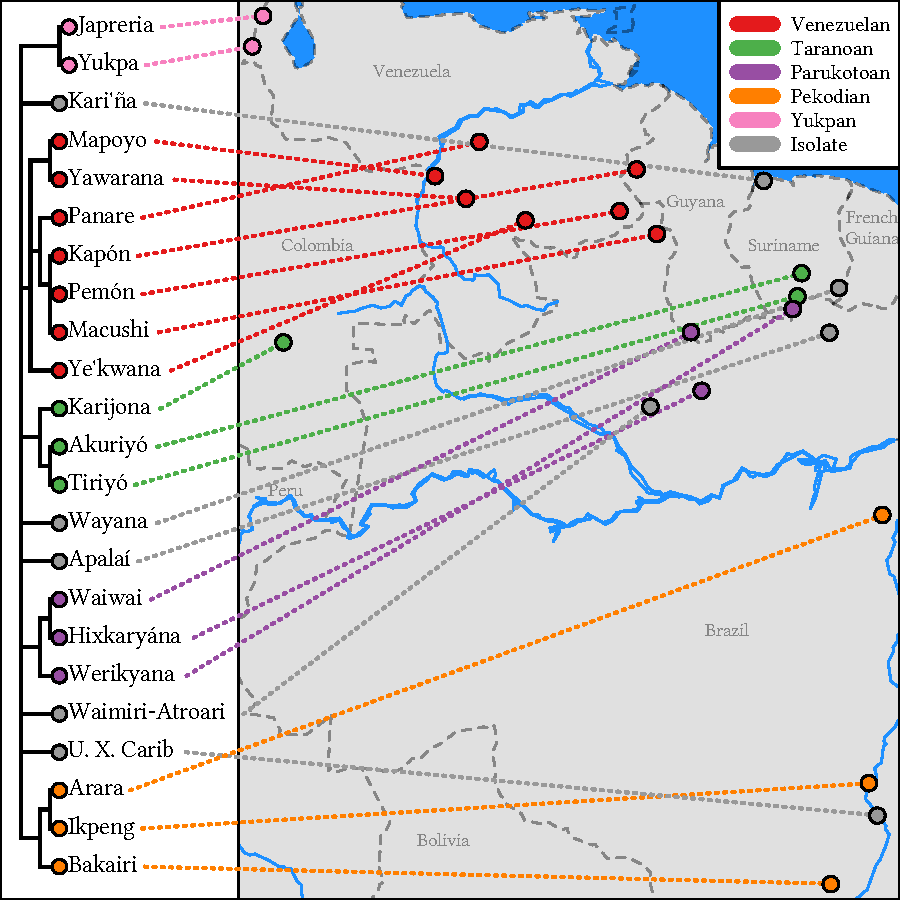
\includegraphics{floats/genealogical_map}
	\caption{The Cariban language family}
	\label{fig:phylomap}
\end{figure}

\begin{table}[htbp]
\centering
\caption[Some \hixka verbs]{Some \hixka verbs \parencites[150, 510, 511, 513, 520]{howard2001wrought}[197, 198]{hixkaryanaderby1985}}
\label{tab:hixintro}
\begin{tabular}[t]{@{}llllll@{}}
\mytoprule
{} &     \qu{to fall} &  \qu{to be afraid} &          \qu{to walk} & \qu{to cut self} &    \qu{to be} \\
\mymidrule
\gl{1}   &  \obj{k-ehurka-} &  \obj{k-oserʲehɨ-} &  \obj{k-atarʲeknohɨ-} &   \obj{k-atama-} &  \obj{w-eʃe-} \\
\gl{2}   &  \obj{m-ehurka-} &  \obj{m-oserʲehɨ-} &  \obj{m-atarʲeknohɨ-} &   \obj{m-atama-} &  \obj{m-eʃe-} \\
\gl{1+2} &  \obj{t-ehurka-} &  \obj{t-oserʲehɨ-} &  \obj{t-atarʲeknohɨ-} &   \obj{t-atama-} &  \obj{t-eʃe-} \\
\gl{3}   &  \obj{ɲ-ehurka-} &  \obj{n-oserʲehɨ-} &  \obj{n-atarʲeknohɨ-} &   \obj{n-atama-} &  \obj{n-eʃe-} \\
\mybottomrule
\end{tabular}
\end{table}
\begin{table}
\centering
\caption[Some \trio verbs]{Some \trio verbs \parencites[292, 294]{triomeira1999}[274]{triocarlin2004}}
\label{tab:triintro}
\begin{tabular}[t]{@{}llllll@{}}
\mytoprule
{} &      \qu{to sleep} & \qu{to see self} & \qu{to bathe (\gl{intr})} &     \qu{to yawn} &     \qu{to go} \\
\midrule
\gl{1}   &    \obj{t-əənɨkɨ-} &    \obj{t-əene-} &              \obj{s-epɨ-} &  \obj{s-entapo-} &  \obj{wɨ-tən-} \\
\gl{2}   &    \obj{m-əənɨkɨ-} &    \obj{m-əene-} &              \obj{m-epɨ-} &  \obj{m-entapo-} &  \obj{mɨ-tən-} \\
\gl{1+2} &  \obj{kɨt-əənɨkɨ-} &    \obj{k-əene-} &             \obj{ke-epɨ-} &  \obj{k-entapo-} &  \obj{kɨ-tən-} \\
\gl{3}   &    \obj{n-əənɨkɨ-} &    \obj{n-əene-} &              \obj{n-epɨ-} &  \obj{n-entapo-} &  \obj{nɨ-tən-} \\
\bottomrule
\end{tabular}
\end{table}

Some languages show a small group of verbs with a divergent first person inflection.
This is illustrated for \hixka in \cref{tab:hixintro},\footnote{The presence of a \gl{1+2} person value implies that of a \gl{1+3} value.
This is usually expressed with a free pronoun combined with third person morphology in Cariban languages, so it is not represented as a distinct value in the paradigms we show.
In \cref{tab:hixintro} and other paradigm tables, we omit any TAM suffixes found in the original forms found in the literature, since a) our focus lies on the prefixes and stems, and b) full paradigms containing the same TAM suffix are rarely found.
Further, we use standard IPA symbols in our transcription of Cariban languages, with the exception of coronal rhotics, which we simply represent with \ort{r}, rather than \ort{ɽ} for \wayana or \ort{ɾ̠} for \maqui etc.
In languages with strong morphophonological processes and/or subphonemic orthography we show the original transcription in an additional surface line when presented in interlinearized examples.
We follow \textcite{gildea2018reconstructing} in using \ort{ə} for the proto-vowel reconstructed by \textcite{meira2005southern}, although it was likely more back \parencite{gildea2010story}.
Glossing abbreviations: }%\glossingAbbrevsComma.
which shows person paradigms for four verbs, all members of the \gl{s_a_} inflectional class.
In this language, the verb \qu{to be} diverges in its first person marker (\obj{w-}), contrasting with other \gl{s_a_} verbs like \qu{to fall}, which have \obj{k(ɨ)-}.
A similar pattern can be found in \trio, where the verb \qu{to go} has a first-person prefix \obj{wɨ-} while other \gl{s_a_} verbs have a prefix with phonologically conditioned allomorphs \envr{\obj{t-}}{\obj{ə}} and \envr{\obj{s-}}{\obj{e}} \pcref{tab:triintro}.
In both languages, the inflectional patterns of the verbs on the left of the table is representative for the vast majority of \gl{s_a_} verbs.
%In both languages, there are only a few other verbs inflected identically to the divergent ones on the right; for example, the first-person form of \trio \qu{to be} is \obj{w-ei-} \parencites[339]{triomeira1999}.

In the literature, such divergent verbs have been identified for \hixka \parencite[188]{hixkaryanaderby1985}, \waiwai \parencite[90]{gildea1998}, the three Taranoan languages \parencite[112--115]{meira1998proto}, \bakairi \parencite{meira2003bakairi}, and \arara \parencite[153]{alves2017arara}.
In a language-particular synchronic analysis, these verbs and their first person prefixes may be considered to be \textsc{irregular}, contrasting with regular prefixes, like \hixka \obj{k(ɨ)-} and \trio \obj{t-}/\obj{s-}, on regular verbs.
However, there is no widely accepted definition of irregularity \parencite{stolz2012introduction}, and many stricter definitions \parencite[][e.g.]{haspelmath2010understanding} require the pattern to occur at a single place in the grammar.
For such approaches, these verbs simply belong to a small inflectional (sub-)class, an analysis suggested for the Pekodian languages \bakairi and \arara \parencites[4]{meira2003bakairi}[149]{alves2017arara}.

Regardless of the synchronic analysis, the reason for these inflectional patterns can be found in the diachrony of the languages in question.
The purpose of this paper is to approach the patterns from a comparative perspective and to provide a unifying diachronic account, for which we first introduce the main clause verbal person marking system of \PC, showing that irregular verbs are conservative \pcref{sec:pc_person}.
That system was subject to many different kinds of innovations, one of which is responsible for  the irregular first person forms \pcref{sec:extensions_intro}.
A particular component of the system, the distinction between \gl{s_a_} and \gl{s_p_} verbs, played a major role in the developments under discussion and is the topic of \cref{sec:split}.
\cref{sec:outlook} summarizes the main points of this section and provides an outlook for the following sections.


% analyses:
%\begin{inlinelist}
%	\item special copula prefix \parencite[188]{hixkaryanaderby1985}
%	\item inflectional subclass \parencites[149]{alves2017arara}[4]{meira2003bakairi}
%	\item \dbqu{exceptional cases} \parencite[293]{triomeira1999}
%	\item phonologically conditioned allomorphs \parencites[139]{meira2006syntactic}{meira2003primeras}[189]{hixkaryanaderby1985}
%	\item not discussed \parencites{waiwaihawkins1998}{ikpengpacheco2001}{alves2013verbo}{pacheco2003intransitivos}
%\end{inlinelist}.
%meira: non-detransitivized verbs
%alves: non-detransitivized verbs (as a consequence, o-initial)



%\subsection{Cariban verbal person marking and marker extensions}
%\label{sec:background}
%The archaic first person markers investigated in this paper are the result of incomplete person marker extensions, i.e., modifications to the ancestral prefix system that did not affect the whole lexicon.
%To provide readers with the necessary background, we first introduce said ancestral system \pcref{sec:pc_person}, then the peculiarities of the Cariban split-\gl{s} system \pcref{sec:split}, and finally the concept of person marker extensions \pcref{sec:extensions_intro}.

\subsection{\PC verbal person marking and conservative verbs}
\label{sec:pc_person}
\PC is reconstructed by \textcite{gildea1998} as using a person paradigm called \setone in its independent verb forms, shown in \cref{tab:pcpers}.
The choice of person marker in transitive verbs can be characterized as being conditioned by a basic person hierarchy \fbox{\gl{1}/\gl{2} > \gl{3}}.
The locuphoric markers had two forms, an \gl{a}-oriented one for direct (\gl{sap}>\gl{3}) scenarios and a \gl{p}-oriented one for inverse (\gl{3}>\gl{sap}) scenarios.
There was a single aliophoric marker \rc{n(i)-}, which only surfaced in nonlocal (\gl{3}>\gl{3}) scenarios, without morphologically expressed distinctions between different third person referents.
Local scenarios were expressed in a non-transparent manner, both using the \gl{1+2} prefix \rc{k-}.

\begin{table}
	\centering
	\caption[\PC \setone (main clause) person markers]{\PC \setone (main clause) person markers \parencites[495]{meira2010origin}[497]{gildea2016referential}}
	\label{tab:pcpers}
	\begin{subtable}[b]{.49\linewidth}
		\caption{Transitive}
		\label{tab:pctrans}
		\centering
		\begin{tabular}{@{}lllll@{}}
			\mytoprule
			\gl{a}/\gl{p}&		\gl{1}	&	\gl{2}		&	\gl{1+2}	&	\gl{3}	\\
			\mymidrule
			\gl{1}	&		&	\rc{k-}	&				&	\rc{t(i)-}		\\	
			\gl{2}	&	\rc{k-}			&&				&	\rc{m(i)-}		\\
			\gl{1+2}&		&				&				&	\rc{kɨt(i)-}		\\
			\gl{3}	&	\rc{u(j)-}	&	\rc{ə(j)-}	&	\rc{k-}			&	\rc{n(i)-}		\\
			\mybottomrule
		\end{tabular}
	\end{subtable}%
	\begin{subtable}[b]{.49\linewidth}
		\caption{Intransitive}
		\label{tab:pcintrans}
		\centering
		\begin{tabular}{@{}lll@{}}
			\mytoprule
			& \gl{s_a_} & \gl{s_p_}  \\
			\mymidrule
			\gl{1} & \rc{w-} & \rc{u(j)-} \\
			\gl{2} & \rc{m-} & \rc{ə(j)-}\\
			\gl{1+2} & \rc{kɨt-} & \rc{k-}\\
			\gl{3} & \rc{n-} & \rc{n(i)-}\\
			\mybottomrule
		\end{tabular}	
	\end{subtable}
\end{table}

Formally identical or etymologically related markers occured in intransitive verbs, which showed a split-\gl{s} system \pcref{tab:pcintrans}.
That is, \gl{s_a_} verbs took similar markers as the \gl{a}-oriented ones in transitive verbs, with the exception of first person (\gl{1}>\gl{3} \rc{t(i)-} vs \gl{1}\gl{s_a_} \rc{w-}), as well as the absence of \rc{i} after all \gl{s_a_} prefixes.
On the other hand, \gl{s_p_} verbs took markers fully identical to the \gl{p}-oriented ones.
The third person marker in \gl{s_p_} verbs was identical to the one in \gl{3}>\gl{3} scenarios (\rc{n(i)-)}.

Equipped with this knowledge about the ancestral system, it becomes clear that the divergent \hixka and \trio forms in \cref{tab:hixintro,tab:triintro} behave irregularly because they preserve the original \PC \gl{1}\gl{s_a_} prefix \rc{w-}; they are therefore \textsc{conservative}.
They contrast with regular \gl{s_a_} verbs, which are innovative in both languages.
The reflexes of \rc{w-} may be considered \textsc{relics}, old and restricted to specific lexically conditioned contexts, contrasting with the innovative prefixes found elsewhere.
These verbs and their prefixes are comparable with the few English nouns like \obj{ɒks}, which preserve the old plural suffix \obj{-ən}.
It, too, was once more widespread, being the normal plural suffix of the weak inflection, compare German \obj{ɔks-n} \qu{ox-en}, \obj{naːmə-n} \qu{name-s}, \obj{haːzə-n} \qu{hare-s}, \obj{bɛːʁ-ən} \qu{bear-s}.
Since the irregular \hixka and \trio prefixes are conservative and the regular prefixes are innovative, the next question to be addressed is where these new prefixes came from.


%\begin{table}
\centering
\caption[Some \maqui verbs]{Some \maqui verbs \parencites[98, 180, 183, 223, 224, 292, 363]{maquiritaricaceres2011}}
\label{tab:makintro}
\begin{tabular}[t]{@{}lllll@{}}
\mytoprule
{} &            \qu{to eat} & \qu{to arrive} &    \qu{to go} &   \qu{to be} \\
\midrule
\gl{1}   &  \obj{w-ətəwasint͡ʃə-} &  \obj{w-əʔrɨ-} &  \obj{w-ɨtə-} &  \obj{w-ei-} \\
\gl{2}   &  \obj{m-ətəwasint͡ʃə-} &  \obj{m-əʔrɨ-} &  \obj{m-ɨtə-} &  \obj{m-ei-} \\
\gl{1+2} &  \obj{k-ətəwasint͡ʃə-} &  \obj{k-əʔrɨ-} &  \obj{k-ɨtə-} &  \obj{k-ei-} \\
\gl{3}   &  \obj{n-ətəwasint͡ʃə-} &  \obj{n-əʔrɨ-} &  \obj{n-ɨtə-} &  \obj{n-ei-} \\
\bottomrule
\end{tabular}
\end{table}

\subsection{Person marker extensions in intransitive verbs}
\label{sec:extensions_intro}
In his discussion of the \PC split-\gl{s} system and reconstruction of the intransitive person prefixes, \textcite[88--96]{gildea1998} shows that the system has undergone many different modifications in various languages.
The main mechanism of change leading to these modifications are \textbf{person marker extensions}, i.e. the use of verbal person prefixes being extended to contexts previously occupied by other prefixes.
%\footnote{
%In principle, one could also imagine a scenario in which verbs of one of the classes are gradually replaced with innovative verbs from the other class, as suggested for \panare by \textcite[225]{meira2000split}.
%However, the verbs Meira sampled came from the \emp{A}-section of \posscite{mattei1994diccionario} dictionary \perscommpar{Spike Gildea}, and \obj{at-}\slash{}\obj{at͡ʃ-}\slash{}\obj{as-} is a frequent reflex of \detrz in \panare, meaning that many \gl{s_a_} verbs are \obj{a}-initial, thus explaining the 80:40 \gl{s_a_}:\gl{s_p_} ratio in Meira's sample.
%Thus, the hypothesis that \panare has largely replaced \gl{s_p_} with \gl{s_a_} verbs remains to be thoroughly tested.
%For the moment, the most likely scenario leading to the eventual loss of the split-\gl{s} system involves markers being extended to new verbs.}
There have been many different person marker extensions in Cariban languages, and some are still ongoing.
This is illustrated by \textcite{gildea1998}, using the three Parukotoan languages as an example.
Apart from segmental changes to individual morphemes, the following innovations happened in the \setone paradigm in Parukotoan:

\begin{enumerate}
	\item \PPar \begin{enumerate}
		\item \gl{1}\gl{s_a_} \rc{w-} to \gl{1}>\gl{3}
		\item \gl{1+2} \rc{k-} to \gl{1}\gl{s_p_} (completed in \PWai, ongoing in \kaxui)
		\item \gl{1+2} \rc{kɨt-} to \gl{1+2}\gl{s_p_} (completed in \PWai, ongoing in \kaxui)
	\end{enumerate}
	\item \PWai \begin{enumerate}
		\item \gl{1}\gl{s_p_} \rc{k-} to \gl{1}\gl{s_a_}
		\item innovative \rc{owɨro j-} \qu{\gl{1}\gl{pro} \gl{lk}} for \gl{1}\gl{p}
	\end{enumerate}
	\item \waiwai \begin{enumerate}
		\item \gl{2}\gl{s_a_} \obj{m-} to \gl{2}\gl{s_p_}\end{enumerate}
\end{enumerate}
%
All innovations are person marker extensions except 2b, which combined a pronoun with the linker \rc{j-}.
They are printed in bold in \cref{fig:par_ext}, which reproduces \posscite{gildea1998} tables as a tree diagram, with adapted transcription and an additional \kaxui \gl{1}\gl{s_p_} marker ∅/\obj{j-} \perscommpar{Spike Gildea}.
%
\begin{figure}[hbt]
	\centering
	\setlength{\tabcolsep}{2pt}
	\fbox{\begin{tikzpicture}[
		every node/.append style={align=center},
		level distance=80pt,
		]
		\Tree[.{\PC{}\pcone}
		[.{\PPar{}\ppone}
		{\kaxui{}\kaxone}
		[.{\PWai{}\pwone}
		{\hixka{}\hixone}
		{\waiwai{}\waione}
		]
		]
		]
	\end{tikzpicture}}
	\caption{Person marking extensions in Parukotoan, after \textcite[94]{gildea1998}}
	\label{fig:par_ext}
\end{figure}
%
\hixka has preserved split-\gl{s} only in the second person prefixes, while \kaxui still shows the variation in the first person and \gl{1+2} prefixes that is reconstructible to \PPar.
\waiwai, on the other hand, has lost the system entirely, which notably happened via distinct innovations at three different diachronic stages.
%In this case, the loss of the inflectional classes also entailed the loss of the other morphological traces of the split-\gl{s} system.
%That is, the \gl{s_a_} class marker \rc{w-} \pcref{sec:split} was lost in \waiwai, as evidenced by the contrast between the \waiwai and \kaxui deverbal forms in \exref{wailoss.wai-158} and \exref{wailoss.kax-138}.
%Similarly, the \gl{2}\gl{s_p_} prefix \obj{a-} was extended to imperatives of (former) \gl{s_a_} verbs \exref[wailoss.wai-112]{wailoss.hix-43}, but only C-initial ones \parencite[62]{waiwaihawkins1998}.


%Such extensions, often only affecting one person value at a time, and the eventual loss of split-\gl{s} are not entirely unexpected, given that the system lacks any semantic basis.

\textcite{gildea1998} discusses person marker extensions in the context of the loss of the split-\gl{s} system and the accompanying changes to indexing alignment; for our story of conservative verbs we will zoom in on a particular aspect of these extensions.
To begin, we argue that they took place via lexical diffusion, characterized as a type of extension by \textcite[106--115]{harris1995historical}; this hypothesis is supported by three facts.
First, the variation in first person and \gl{1+2} prefixes described above for \kaxui is not completely free.
Rather, some verbs only allow for example first person \obj{k-}, but not \obj{j-}, while others can occur with both, which is the expected pattern in a lexical diffusion scenario.
In addition, this is speaker-dependent \perscommpar{Spike Gildea}, which is what one would expect from a change in progress.
%todo maybe put in GOOD kaxui data
Second, while there is no detailed diachronic scenario for the switch of \gl{1}>\gl{3} \rc{t-} and \gl{1}\gl{s_a_} in the Tiriyoan languages \pcref{sec:taranoan}, \textcite[111--112]{meira1998proto} convincingly argues that it must have happened gradually rather than instantaneously, and entailed both markers spreading at the same time.
Whether this gradual switch was along ordered lines or not, lexical diffusion must have played a role.

Our third argument in favor of the lexical diffusion scenario brings us back to the conservative \hixka and \trio forms in \cref{tab:hixintro,tab:triintro}.
In both cases, the innovative \gl{1}\gl{s_a_} prefixes were introduced by a person marker extension spreading via lexical diffusion.
We interpret the continued presence of the old \gl{1}\gl{s_a_} prefix in a few verbs as the extension stopping short of these verbs, rather than affecting all targets (\gl{s_a_} verbs).
In our family-wide investigation of person marker extensions, we identified 19 distinct extensions affecting intransitive verbs, and found 6 of them to be incomplete.
These incomplete extensions have left between 1 and 7 conservatively inflected verbs in 9 Cariban languages. %, marked with bold print in \cref{fig:caribantree}.

Interestingly, all six extensions featured innovative first person markers on \gl{s_a_} verbs.
While extensions occurred with other person values as well, they never affected \gl{s_a_} verbs, only \gl{s_p_} ones, and they always affected all potential targets.
Illustrative examples for complete extensions are shown in \cref{tab:completed}: the extension of \gl{1+2}\gl{s_a_} \obj{s(ɨ)-} (< \rc{kɨt-}) to \gl{s_p_} verbs in \apalai \pcref{tab:apalai}, of \gl{2}\gl{s_a_} \obj{m(ɨ)-} in to \gl{s_p_} verbs in \panare \pcref{tab:panare},\footnote{The presence of the third person marker \obj{n-} for \gl{1+2} is due to the wholesale loss of that inflectional value.} or the extension of the entire \gl{s_a_} set to \gl{s_p_} verbs in \waimiri \pcref{tab:waimiri}. %, as well as the extension of \rc{k-} to \gl{1}\gl{s_p_} and of \rc{tɨt-} to \gl{1+2}\gl{s_p_} in \PWai \pcref{fig:par_ext}.
The markedly different behavior of \gl{s_a_} and \gl{s_p_} verbs with regards to the extent of extensions affecting them points to the split-\gl{s} system playing some role, so we will discuss its main properties in \cref{sec:split}.
This will also give readers an idea how it is possible for the \gl{s_a_}/\gl{s_p_} distinction to be lost only for a single person, or for \gl{s_p_} verbs to take on \gl{s_a_} markers with apparent semantic impunity.

\begin{table}
	\caption[Some examples for completed extensions]{Some examples for completed extensions \parencite[90--92]{gildea1998}}
	\label{tab:completed}
	\begin{subtable}[h]{0.24\textwidth}
		\centering
		\caption{\apalai}
		\label{tab:apalai}
		\begin{tabular}{@{}lll@{}}
			\mytoprule
			& \gl{s_a_} & \gl{s_p_}\\
			\mymidrule
			\gl{1} & ∅/\obj{ɨ-} & \obj{ɨ-}/\obj{j-}\\
			\gl{2} & \obj{m(ɨ)-} & \obj{o-}\\
			\gl{1+2} & \multicolumn{2}{c}{\emp{\obj{s(ɨ)-}}}\\
			\gl{3} & \multicolumn{2}{c}{\obj{n(ɨ)-}}\\
			\mybottomrule
		\end{tabular}
	\end{subtable}
	\hfill
	\begin{subtable}[h]{0.24\textwidth}
		\centering
		\caption{\panare}
		\label{tab:panare}
		\begin{tabular}{@{}lll@{}}
			\mytoprule
			& \gl{s_a_} & \gl{s_p_}\\
			\mymidrule
			\gl{1} & \obj{w(ɨ)-} & ∅/\obj{j-}\\
			\gl{2} & \multicolumn{2}{c}{\emp{\obj{m(ɨ)-}}}\\
			\gl{1+2} & \multicolumn{2}{c}{\obj{n(ɨ)-}}\\
			\gl{3} & \multicolumn{2}{c}{\obj{n(ɨ)-}}\\
			\mybottomrule
		\end{tabular}
	\end{subtable}
	\hfill
	%\begin{subtable}[h]{0.24\textwidth}
	%\centering
	%\caption{\pemon}
	%\label{tab:pemon}
	%\begin{tabular}{@{}lll@{}}
	%\mytoprule
	%& \gl{s_a_} & \gl{s_p_}\\
	%\mymidrule
	%\gl{1} & \multicolumn{2}{c}{\emp{∅}}\\
	%\gl{2} & \multicolumn{2}{c}{\emp{\obj{m-}}}\\
	%\gl{1+2} & \multicolumn{2}{c}{\obj{n-}}\\
	%\gl{3} & \multicolumn{2}{c}{\obj{n-}}\\
	%\mybottomrule
	%\end{tabular}
	%\end{subtable}
	%\hfill
	\begin{subtable}[h]{0.24\textwidth}
		\centering
		\caption{\waimiri}
		\label{tab:waimiri}
		\begin{tabular}{@{}ll@{}}
			\mytoprule
			& \gl{s}\\
			\mymidrule
			\gl{1} & \emp{\obj{w(ɨ)-}/\obj{i-}}\\
			\gl{2} & \emp{\obj{m(ɨ)-}}\\
			\gl{1+2} & \emp{\obj{h(ɨ)-}}\\
			\gl{3} & \obj{n-}/∅\\
			\mybottomrule
		\end{tabular}
	\end{subtable}
\end{table}

\subsection{The Cariban split-\gl{s} system}
\label{sec:split}
As seen in \cref{sec:pc_person}, the \PC distinction between \gl{s_a_} and \gl{s_p_} verbs was instantiated by two inflection classes within the \setone person paradigm, but this was not the only inflectional difference:
%\begin{inlinelist}
%	\item presence vs absence of the \gl{s_a_} marker \rc{w-}
%	\item absence vs presence of the second person prefix \rc{ə(j)-} in imperatives
%	\item presence vs absence of a derivational detransitivizing prefix
%\end{inlinelist}.
%
Many languages show an \gl{s_a_} class marker in deverbalized forms, originating in \PC \rc{w-}.\footnote{See \textcite[227]{meira2000split}, who identifies reflexes of this morpheme as having \dbqu{no purpose other than being \qu{class markers}, without any obvious semantic or functional load}.}
With \gl{s_a_} verbs, \rc{w-} occurred immediately between the possessive prefixes and the verb stem, while \gl{s_p_} verbs took the bare prefixes.
Reflexes of \rc{w-} in languages from different branches are illustrated in \cref{tab:participles,tab:nominalizations} for participles and nominalizations.%
%
\begin{table}
\centering
\caption[Participles of \gl{s_a_} and \gl{s_p_} verbs]{Participles of \gl{s_a_} and \gl{s_p_} verbs \parencites[39]{schuring2018kaxuyana}[118, 207]{alves2017arara}[333-334]{triomeira1999}[400]{wayanatavares2005}[35]{koehn1986apalai}[kuruaz-154]{koehns1994textos}[430, 433]{hoff1968carib}[232, 244]{panarepayne2013}}
\label{tab:participles}
\begin{tabular}[t]{@{}lll@{}}
\mytoprule
Language &                               \gl{s_a_} &                        \gl{s_p_} \\
\mymidrule
\kaxui  &         \obj{t-ehurka-t͡ʃe} \qu{fallen} &       \obj{tɨ-jaʔ-so} \qu{burnt} \\
\arara  &         \obj{t-\emp{o-}ep-te} \qu{come} &      \obj{t-oregrum-te} \qu{sad} \\
\trio   &    \obj{tɨ-\emp{w-}əturu-e} \qu{talked} &       \obj{t-əpəə-se} \qu{tired} \\
\wayana &     \obj{tə-\emp{w-}epɨ-he} \qu{bathed} &    \obj{t-onopɨ-he} \qu{painted} \\
\apalai &        \obj{t-\emp{o-}ɨto-se} \qu{gone} &   \obj{t-ɨhto-se} \qu{gone down} \\
\kalina &  \obj{tu-\emp{w-}oʔka-se} \qu{come out} &       \obj{t-okari-se} \qu{told} \\
\panare &  \obj{t-\emp{o-}tatɨhpə-se} \qu{wailed} &  \obj{tɨ-sɨrɨke-t͡ʃe} \qu{tired} \\
\mybottomrule
\end{tabular}
\end{table}%
%
\begin{table}
\centering
\caption[Nominalizations of \gl{sa} and \gl{sp} verbs]{Nominalizations of \gl{sa} and \gl{sp} verbs \parencites[49, 74]{schuring2018kaxuyana}[97]{alves2017arara}[246]{triomeira1999}[130, 409]{wayanatavares2005}[90]{koehn1986apalai}[ner2-003]{koehns1994textos}[135, 392]{hoff1968carib}[390]{panarepayne2013}[23]{mattei1994diccionario}}
\label{tab:nominalizations}
\begin{tabular}[t]{@{}lll@{}}
\mytoprule
Language &                                         \gl{sa} &                                             \gl{sp} \\
\mymidrule
\kaxui  &       \obj{o-\emp{w-}ehurka-tpɨrɨ} \qu{your fall} &            \obj{o-onenmehɨ-tpɨrɨ} \qu{your waking up} \\
\arara  &        \obj{\emp{w-}orik-tubo} \qu{dancing place} &              \obj{ereŋmɨ-tpo} \qu{killing instrument} \\
\trio   &   \obj{ji-\emp{w-}əturu-to} \qu{(for) my talking} &              \obj{j-emamina-to} \qu{(for) my playing} \\
\wayana &          \obj{ɨ-\emp{w-}əturu-topo} \qu{my story} &        \obj{j-ɨnɨkɨ-topo} \qu{my object for sleeping} \\
\apalai &            \obj{j-epɨ-topo} \qu{my bathing place} &   \obj{j-enuru-topõ-pɨrɨ} \qu{the place of my birth} \\
\kalina &  \obj{a-\emp{w-}ekupi-rɨ} \qu{your taking a bath} &    \obj{aj-ereʔna-{\normalfont ∅}} \qu{your fainting} \\
\panare &     \obj{j-\emp{u-}t͡ʃireema-n} \qu{their eating} &  \obj{tj-arunkampətɨ-n} \qu{his hair standing on end} \\
\mybottomrule
\end{tabular}
\end{table}%
%
\begin{table}[htbp]
\centering
\caption[Imperatives of \gl{s_a_} and \gl{s_p_} verbs]{Imperatives of \gl{s_a_} and \gl{s_p_} verbs \parencites[44, 89]{derbyshire1965textos}[161]{alves2017arara}[323]{triomeira1999}[227]{wayanatavares2005}[62]{koehn1986apalai}[Mopo/20]{koehns1994textos}[190]{hoff1968carib}[5, 17]{mattei1994diccionario}}
\label{tab:imperatives}
\begin{tabular}[t]{@{}lll@{}}
\mytoprule
Language &                         \gl{s_a_} &                             \gl{s_p_} \\
\mymidrule
\hixka  &          \obj{omoh-ko} \qu{come!} &  \obj{\emp{oj-}okajɨm-ko} \qu{go up!} \\
\arara  &  \obj{odotpot-ko} \qu{come back!} &      \obj{\emp{o-}alum-ko} \qu{jump!} \\
\trio   &          \obj{epɨ-kə} \qu{bathe!} &   \obj{\emp{ə-}eremina-kə} \qu{sing!} \\
\wayana &         \obj{əməm-kə} \qu{enter!} &    \obj{\emp{əw-}eremi-kə} \qu{sing!} \\
\apalai &           \obj{otuʔ-ko} \qu{eat!} &      \obj{\emp{o-}nɨʔ-ko} \qu{sleep!} \\
\kalina &         \obj{oʔmaʔ-ko} \qu{stop!} &   \obj{\emp{aj-}awon-ko} \qu{get up!} \\
\panare &            \obj{ape-ʔ} \qu{flee!} &             \obj{ahpən-kə} \qu{jump!} \\
\mybottomrule
\end{tabular}
\end{table}
%
The distinction between \gl{s_a_} and \gl{s_p_} was also borne out in imperatives, where the latter took the \gl{p}-oriented second person prefix \rc{ə(j)-}, while the former received no prefix (both suffixed with \rc{-kə}).
This is illustrated with reflexes in various modern languages in \cref{tab:imperatives}.
Both the \gl{s_a_} marker \rc{w-} and the prefix pattern in imperatives have been lost in some languages, but are reconstructible to \PC.
%However, there was one further property uniting most \gl{s_a_} verbs, not based on inflectional morphology.


In the modern languages maintaining the split-\gl{s} system, mismatches between the semantics of verbs and their \gl{a}- or \gl{p}-oriented inflectional morphology are common, exemplified with \kalina data in \exref[kar1]{kar2}.

\pex<kar1> \kalina
\a<kar-60>
\begingl
\gla mi-kupi-ja//
\glb \gl{2}>\gl{3}-bathe-\gl{prs}//
\glft \qu{You bathe him/her.} \parencite[][160]{hoff1968carib}//
\endgl
\a<kar-62>
\begingl
\gla a-kupi-ja//
\glb \gl{3}>\gl{2}-bathe-\gl{prs}//
\glft \qu{S/he bathes you.} \parencite[][63]{yamada2011evidentiality}//
\endgl
\xe
%
In \exref{kar1}, the choice between the second person \gl{a}- and \gl{p}-oriented markers \obj{mi-} and \obj{a-} depends on the scenario:
The transitive verb \obj{kupi} \qu{to bathe} takes \obj{mi-} in \gl{2}>\gl{3} scenarios \exref{kar1.kar-60}, but \obj{a-} in \gl{3}>\gl{2} scenarios \exref{kar1.kar-62}.
The intransitive verbs in \exref{kar2} show the same person markers, but the choice of marker depends on the verb, rather than semantics.

\pex<kar2> \kalina
\a<kar-59>
\begingl
\gla sipi tɨnka-rɨ m-ekema-non hen//
\glb net pull-\gl{nmlz} \gl{2}-be.afraid-\gl{prs}.\gl{uncert} eh?//
\glft \qu{You're afraid to pull up the net, aren't you? } \parencite[][253]{courtz2008carib}//
\endgl
\a<kar-61>
\begingl
\glpreamble aya:woiya //
\gla aj-awomɨ-ja//
\glb \gl{2}-get.up-\gl{prs}//
\glft \qu{You are getting up.} \parencite[][167]{hoff1968carib}//
\endgl
\xe
%
Thus, \obj{ekema} \qu{to be afraid} takes an \gl{a}-oriented marker, since it is an \gl{s_a_} verb \exref{kar2.kar-59}, while the \gl{s_p_} verb \obj{awomɨ} \qu{to get up} takes a \gl{p}-oriented marker \exref{kar2.kar-61}.
In both cases, the prefix does not appear to contribute to the semantics of the predicate, since there are clear mismatches:
\qu{to be afraid} with an \dbqu{agentive} marker can hardly be considered a volitional act, while  \qu{to get up} with a \dbqu{patientive} marker must be considered volitional.
\textcite{meira2000split} takes a sizable corpus of intransitive verbs from \trio, \kalina, \apalai, and \wayana, and categorizes them by applying different criteria commonly encountered in split-\gl{s} systems.
He shows that neither (non\-)activities, % \parencite[210]{meira2000split}, 
(non-)agency, % \citeyearpar[212]{meira2000split}, 
(in-)animacy, % \citeyearpar[213]{meira2000split},
nor Aktionsart % \citeyearpar[215]{meira2000split} 
satisfactorily predict the class membership of intransitive verbs in any of the languages.

Rather, the reason for a verb to take \gl{a}- or \gl{p}-oriented prefixes is (at least diachronically) a morphological one.
\textcite[217--221]{meira2000split} demonstrates that those intransitive verbs which (etymologically) have a detransitivizing prefix are treated as \gl{s_a_} verbs, while essentially all others are \gl{s_p_} verbs:
\begin{quotebox}{\parencite[201]{meira2000split}}
	Almost all verbs in the \gl{s_a_} class are detransitivized forms of transitive verbs, either synchronically (with still exisiting transitive sources) or diachronically (with reconstructible but no longer existing transitive sources)
\end{quotebox}
\textcite[221--223]{meira2000split} also argues that the detransitivizing prefixes are indeed deriving \gl{s_a_} verbs, rather than being inflectional in nature:
\begin{inlinelist}
	\item there are a few underived \gl{s_a_} verbs, with no detransitivizing prefix
	\item \gl{s_a_} verbs can develop irregular semantics compared to their transitive counterparts
	\item it is unpredictable whether the \gl{a} or \gl{p} argument of the underlying transitive verb becomes the \gl{s} of the derived \gl{s_a_} verb
	\item some originally derived \gl{s_a_} verbs have lost their transitive counterparts
	\item \dbqu{basic} concepts are expressed as derivations of more complex concepts, like \qu{to dance (\gl{s_a_})} from \qu{to dance with (\gl{tr})}
\end{inlinelist}.
He also notes that this leads to an inflectional split not based in meaning, but rather morphology:

\begin{quotebox}{\parencite[226]{meira2000split}}
	Apparently, the morphological behavior of the \gl{s_a_} verb class is an accidental consequence of the fact that detransitivization, as far back as we can reconstruct, entails all the morphology described […] as typical of \gl{s_a_} verbs. The alignment of person-marking prefixes appears not to be driven by any semantic forces in the language; it is as though they were being dragged by the evolution of the reflexive marker.
\end{quotebox}

As for the form of this marker, \textcite[505--512]{meira2010origin} reconstruct two distinct  prefixes for \PC: reciprocal \rc{əte-} and reflexive \rc{e-}, although on verbs their reflexes have been merged in a single morpheme in modern languages.
Modern reflexes of \detrz show a range of meanings, which can all be characterized as \dbqu{detransitive}; this range is illustrated with \trio examples in \exref{triodetrz}.

\ex<triodetrz> \trio \parencites[218--219]{meira2000split}[128, 256]{triomeira1999}\\
\begin{tabular}[t]{@{}llll@{}}
	\\
	\obj{nonta}  & → & \obj{e-nonta}, & \qu{abandon each other}\\
	\qu{abandon} & & \obj{əi-nonta} &  (reciprocal) \\
	\\
	\obj{suka} & → & \obj{e-suka}, & \qu{wash self}\\
	\qu{wash} & & \obj{əi-suka} & (reflexive)\\
	\\
	\obj{pahka} & → & \obj{e-pahka} & \qu{break (\gl{intr})}\\
	\qu{break (\gl{tr})} & & & (anticausative)\\
	\\
	\obj{puunəpɨ} & → & \obj{əh-puunəpɨ}, & \qu{think, meditate}\\
	\qu{think about} & & \obj{əi-puunəpɨ} & (antipassive)\\
\end{tabular}
\xe
%
The morphological variation featured in \qu{to abandon each other} and \qu{to wash self} is due to the mentioned collapse between the two \PC prefixes:
\obj{e-} is a reflex of the reflexive prefix \rc{e-}, while the form \obj{əi-} originates in reciprocal \rc{əte-}.
However, both can occur with either meaning -- at least for these two verbs.
%As mentioned, there are a few \gl{s_a_} verbs that are not derived from transitive verbs, and do not have a reflex of \detrz, either.
%\textcite[221]{meira2000split} characterizes these as very old and exceptional, and counts between 5 and 7 verbs, depending on the language.
%\textcite{gildea2007greenberg} identify 7 such underived \gl{s_a_} verbs as reconstructible to \PC, shown in \cref{tab:underived2007}.
%Many of these verbs will be discussed in \cref{sec:verbs}.

%\begin{table}
	\centering
	\caption[Underived \PC \gl{sa} verbs]{Underived \PC \gl{sa} verbs \parencite[30]{gildea2007greenberg}}
	\label{tab:underived2007}
	\begin{tabular}{@{}lll@{}}
		\mytoprule
		Form & Meaning\\
		\mymidrule
		\rc{tə[mə]} & \qu{to go}\\
		\rc{ətepɨ} & \qu{to come\subs{1}}\\
		\rc{ka[ti]} & \qu{to say}\\
		\rc{əmə[mɨ]} & \qu{to enter}\\
		\rc{eti} & \qu{to dwell, be\subs{2}}\\
		\rc{a[p]} & \qu{to be\subs{1}, say}\\
		\rc{əməkɨ} & \qu{to come\subs{2}}\\
		\mybottomrule
	\end{tabular}
\end{table}


\subsection{Summary and outlook}
\label{sec:outlook}
We identified \gl{s_a_} verbs that irregularly inflect for first person in 9 Cariban languages.
These irregular forms are actually conservative, belonging to a few verbs unaffected by person marker extensions spread via lexical diffusion.
Such conservative forms are only found among the first person forms of  (etymological) \gl{s_a_} verbs.
The goal is to establish what verbs remained unaffected by the individual extensions and to find reasons for their conservativeness, for which we proceed as follows:
The topic of \cref{sec:extensions} are the six incomplete innovations, the innovative markers they introduced, and the verbs they left untouched.
Since these verbs show considerable etymological overlap between languages, they are reconstructed and discussed in more detail in \cref{sec:verbs}.
Finally, we search for factors motivating the resistance of these verbs, discuss the findings and put them in a general context of language change and morphology in \cref{sec:discussion}.